\documentclass[]{article}

\usepackage{pdfpages} 
\usepackage[utf8]{inputenc}
\usepackage[spanish]{babel}
\usepackage[nottoc, numbib]{tocbibind} %bibindex

% Title Page
\title{Título de la propuesta}
\author{Estudiante}

\begin{document}
	
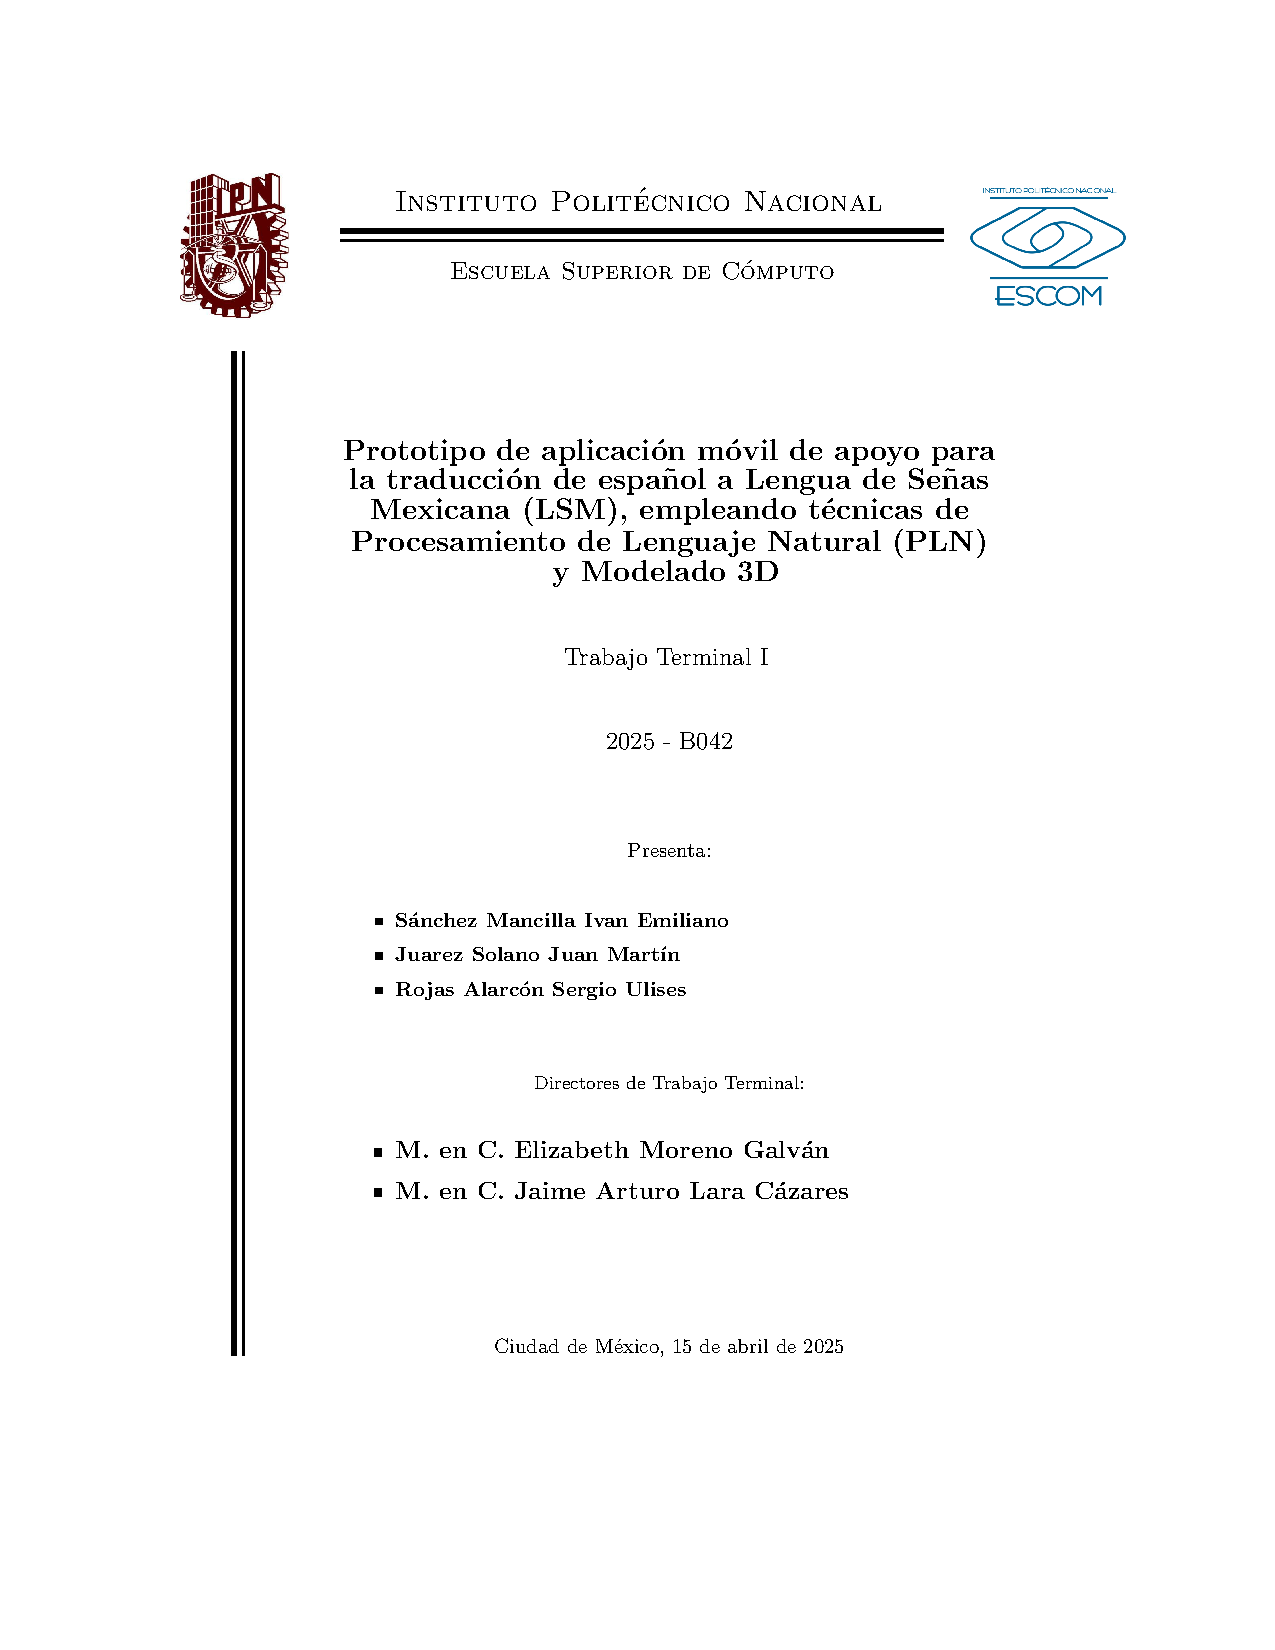
\includepdf[pages={1}]{portada.pdf}
	
%\newpage\null\thispagestyle{empty}\newpage
	
%\maketitle

\begin{abstract}
	Aqui va el resumen. Describir de forma conscisa el problema y que técnicas se pretenden usar para abordarlo. 
\end{abstract}

%\newpage\null\thispagestyle{empty}\newpage

%\addtocontents{toc}{\hfill \textbf{Página} \par}
%\tableofcontents

\section{Introducción}
\subsection{Motivación}
\subsection{Problema}

\section{Trabajo Relacionado}

\section{Propuesta}

\subsection{Hipótesis}

Revisar el libro de \cite{hernandez2018metodologia}.

\subsection{Objetivo General}
\subsection{Metodología}

\subsection{Cronograma}

\section{Avances}

Si es que hay avances aqui debes colocarlos.

\section{Conclusiones}

\bibliographystyle{plain}
\bibliography{referencias}

\end{document}          
